\documentclass[phd, titlesmallcaps, examinerscopy, copyrightpage, foronline]{mqthesis}

% Some typical packages you might use
\usepackage{rotating}  %used to rotate things like pictures or things you \put down
\usepackage{theorem}   %for mathematical theorems and lemmas
\usepackage{bm}  %bold fond inside equations, eg. $\bm{\alpha}$
\usepackage{amsmath,amsfonts,amssymb}
\usepackage{booktabs}  %Makes nice tables in books (sorta like RevTeX can)
\usepackage{pdfsync}   %used to sync pdf output inorder to flip from tex file to pdf and back
 %graphicx is already included in the class file

\ifpdf
    \pdfinfo { /Title  (Title of Thesis)
               /Creator (pdflatex) % probably this
               /Producer (LaTeX with hyperref) % something like this
               /Author (Jeffrey `The Dude' Lebowski the_dude@lebowski.com)
               %/CreationDate (D:20100204000000)  %format D:YYYYMMDDhhmmss
		% if /CreationDate is left out it will default to the file creation date
               /Keywords (Obscure; Fields; Science; White Russians)}
    \pdfcatalog { /PageMode (/UseOutlines) /OpenAction (fitbh)  }
\fi

\begin{document}

\frontmatter

%%%%% Acknowledgements, titlepage, abstract, list of publications
\title{Insert thesis title here}

\ifthenelse{\boolean{foronline}}{
  \author{\href{mailto:the_dude@lebowski.com}{Jeffrey `The Dude' Lebowski}}
  \department{Physics}
}{
  \author{Jeffrey `The Dude' Lebowski}
  \department{Physics}
}


%%%%% Submition date if different from creation date
% \submitdate{March 2010}

% honours students will want to use the keyword honours instead of phd :)
% or override the \degreetext variable with
% something appropriate like:
% \renewcommand{\degreetext}%
% {in partial fulfilment of the Degree of Bachelor of Science with Honours}
% also easy to changes this to be for Masters degrees.

\titlepage

\chapter{Acknowledgements}

I would like to thank Walter for being a great budy even if he is sometimes somewhat misguided. It would also seem apropiate to thank the Russians for vodka, and the cows for milk. The cornerstones of my dietary sustenance.

This thesis is dedicated in memory of my friend Donny who died in a battle with nihilists.

- The Dude abides.

\chapter{List of Publications}

\begin{itemize}
\item[$\bullet$] insert author list \emph{insert paper title}.  (submitted to
	insert journal name)
\item[$\bullet$] insert author list \emph{insert paper title}.  
        insert journal name \textbf{insert volume number}, 
        insert article or page number (insert year)
\end{itemize}


Organisms are routinely faced with the task of making decisions based on partial, unreliable information. Furthermore, not only is the environment noisy, but the computational units 
organisms employ themselves are often faulty and noisy, such as the neurons of the animal nervous system. There is a crucial difference, though: while the organism can only act
indirectly on its environment, its sensory organs are under its direct control through adaptation. Here I thus consider how a population of neurons can organise itself to allow for optimal information 
processing at its output. I will focus on a model of a rapidly changing environment, which forces the organism to make short-time decisions.\par

In that setting I have provided a number of novel results, extending the framework of population coding to a fully dynamic setting, where a changing environment is decoded from
spike trains in an online fashion. To do so, I have drawn from the theory of stochastic filtering of doubly stochastic point processes. For a dense population of neurons, this
reduces to a Gaussian process regression problem, for which I have obtained closed form relations for the error distribution. The formalism developed also lends itself to a direct 
extension to a control-theoretical setting. Thus I have also developed a criterion for optimal coding
in the case of control problems, and have compared this to the case of estimation previously developed. Interestingly, I have been able to show that the different objective functions
for control and estimation lead to different optimal encoders.\par

The study of optimal coding in populations of neurons is an active fertile area of research. Here I have extended a number of previous findings to the case of online decoding of
dynamic stimuli from point processes. Parallel to that, I have discussed the issue of optimal coding for control, and how it relates to the study of optimal coding in the estimation case.





\tableofcontents
\listoffigures
\listoftables

\mainmatter

%%%%% Introduction
\begin{savequote}[10cm] % this sets the width of the quote
\sffamily
``Forget it, Donny, you're out of your element!'' 
\qauthor{Walter Sobchak - The Big Lebowski}
\end{savequote}

\chapter{Introduction}

This is not a very interesting introduction, however, every thesis probably
needs one.



%%%%% Other chapters in here
\begin{savequote}[10cm] % this sets the width of the quote
\sffamily
``This is not Nam. This is bowling. There are rules!'' 
\qauthor{Walter Sobchak - The Big Lebowski}
\end{savequote}

\chapter{Another Chapter}
\graphicspath{{ch1/}} 


It's likely that you'll need another chapter, so here's a filler just to see
where it will go \cite{sample}. Also here is a figure \ref{lambda}, so
you can see how the \emph{hyperref} package works. Note the
hyperlinking of the citation and figure reference. This will only work if you have the \emph{foronline} option included for the MQThesis document class, at the top of thesis.tex.

\begin{figure}[tbp]  
\begin{center}
\setlength{\unitlength}{1cm}
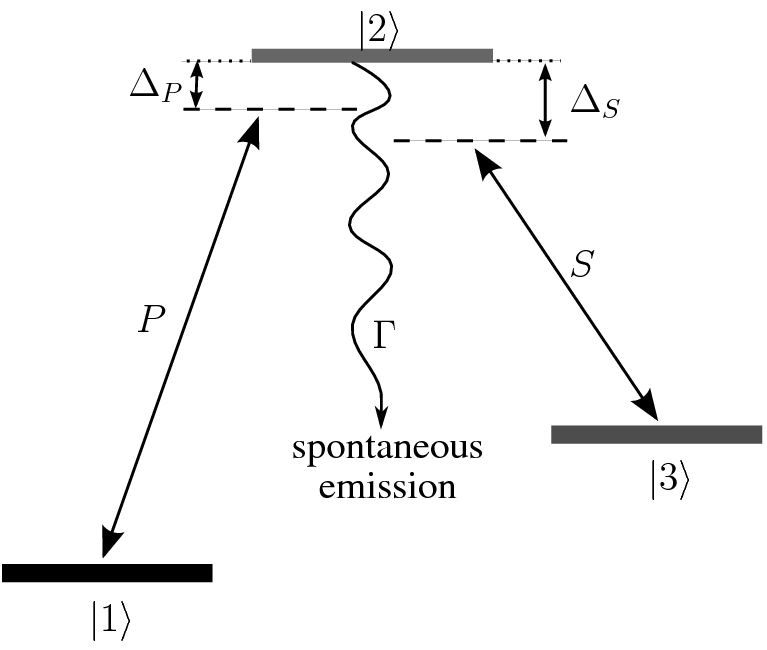
\includegraphics[width=8.4\unitlength]{lambda.png}
\end{center}
\caption{The $\Lambda$-type three-level energy scheme. States
$|1\rangle$ and $|2\rangle$ are coupled by the pump pulse $P$ which has a
detuning $\Delta_P$ from being exactly on resonance.  Similarly states
$|2\rangle$ and $|3\rangle$ are coupled by the Stokes pulse $S$ which has a
detuning $ \Delta_S$. State $|2\rangle$ is short lived with spontaneous emission
occurring out of the system}
\label{lambda}
\end{figure}


%\input{ch2/chap_2}

%%%%% Conclusion
\begin{savequote}[10cm] % this sets the width of the quote
\sffamily
``Yeah, well, you know, that's just, like, your opinion, man.'' 
\qauthor{The Dude - The Big Lebowski}
\end{savequote}

\chapter{Conclusion}

Not a very interesting conclusion, however you'll need one for your thesis.


\appendix

%%%%% Appendix
\chapter{An Appendix}

This is an appendix.  Add anything in here that you need in an appendix.


 
\backmatter

%%%%% List of symbols
% your thesis may not need this, so comment out or delete the following line
\chapter{List of Symbols}

% please change this list to suit your thesis

The following list is neither exhaustive nor exclusive, but may be helpful.
\begin{list}{}{%
\setlength{\labelwidth}{24mm}
\setlength{\leftmargin}{35mm}}
\item[$a$, $b$, $c$, $d$\dotfill] annihilation operators
\item[$a^\dagger$, $b^\dagger$, $c^\dagger$, $d^\dagger$\dotfill] creation
operators
\end{list}


%%%%% Bibliography, in BibTeX format (the references.bib file)
\bibliography{references}

\end{document}
